
%\documentclass[preprint]{acmart}
\documentclass[preprint]{elsarticle}
\journal{Science of Computer Programming}

\usepackage{todonotes}

\usepackage{listings}
\usepackage{xcolor}
\usepackage{siunitx}
\usepackage{tikz-uml}
\usepackage{hyperref}
\hypersetup{pdfauthor={Sylvain Guérin, Jean-Christophe Bach, Antoine Beugnard, Joel Champeau, Salvador Mart\'inez, Guillaume Pollet, Caine Silva}}

\definecolor{codegreen}{rgb}{0,0.6,0}
\definecolor{codegray}{rgb}{0.5,0.5,0.5}
\definecolor{codepurple}{rgb}{0.58,0,0.82}
\definecolor{backcolour}{rgb}{0.95,0.95,0.92}

\lstdefinestyle{mystyle}{
    backgroundcolor=\color{backcolour},   
    commentstyle=\color{codegreen},
    keywordstyle=\color{magenta},
    numberstyle=\tiny\color{codegray},
    stringstyle=\color{codepurple},
    basicstyle=\ttfamily\footnotesize,
    breakatwhitespace=false,         
    breaklines=true,                 
    captionpos=b,                    
    keepspaces=true,                 
    numbers=left,                    
    numbersep=5pt,                  
    showspaces=false,                
    showstringspaces=false,
    showtabs=false,                  
    tabsize=2
}

\lstset{style=mystyle}

\DeclareTextFontCommand{\mytexttt}{\ttfamily\hyphenchar\font=45\relax}

% DRAFT
\newcommand{\ab}[1]{{\color{blue} #1}} % draft mode
\newcommand{\jcb}[1]{{\color{red} #1}} % draft mode
\newcommand{\sg}[1]{{\color{purple} #1}} % draft mode

%\acmPrice{15.00}
%\acmDOI{10.1145/1122445.1122456}
%\acmISBN{978-1-4503-9999-9/18/06}

\begin{document}
\begin{frontmatter}

\title{PAMELA: an annotation-based Java Modeling Framework}

%% Group authors per affiliation:
%\author{Sylvain Guérin, Guillaume Polet, Caine Silva, Joel Champeau}
%\address{ENSTA Bretagne}

%\author{Jean-Christophe Bach, Salvador Martinez, Antoine Beugnard}
%\address{IMT Atlantique}

%% or include affiliations in footnotes:
\author[mymainaddress]{Sylvain Guérin\corref{mycorrespondingauthor}}
\cortext[mycorrespondingauthor]{Corresponding author}
%\ead{firstname.lastname@ensta-bretagne.fr}

\author[mymainaddress]{Guillaume Polet}
%\ead{firstname.lastname@ensta-bretagne.fr}

\author[mymainaddress]{Caine Silva}
%\ead{firstname.lastname@ensta-bretagne.fr}

\author[mymainaddress]{Joel Champeau}
%\ead{firstname.lastname@ensta-bretagne.fr}

\author[mysecondaryaddress]{Jean-Christophe Bach}
%\ead{firstname.lastname@imt-atlantique.fr}

\author[mysecondaryaddress]{Salvador Mart\'inez}
%\ead{firstname.lastname@imt-atlantique.fr}

\author[mysecondaryaddress]{Fabien Dagnat}
%\ead{firstname.lastname@imt-atlantique.fr}

\author[mysecondaryaddress]{Antoine Beugnard}
%\ead{firstname.lastname@imt-atlantique.fr}

\address[mymainaddress]{ENSTA Bretagne, Lab-STICC, UMR 6285, Brest, France}%vérifier si c'est l'affiliation officielle
\address[mysecondaryaddress]{IMT Atlantique, Lab-STICC, UMR 6285, Brest, France}



\begin{abstract}
This article presents PAMELA, an annotation-based Java modeling framework. PAMELA provides a smooth integration between model and code and enables Java developers to handle software development both at conceptual level and at source-code level, without code transformation and/or generation, avoiding round-trip-related issues.

% TODO...

% Parler aussi de Aspect Oriented Programming, Traits programming, Run-time weaving, Semantics Add-On, MOP (Meta Object Protocol) 

\end{abstract}



\begin{keyword}
Model Driven Engineering \sep Object Oriented Programming \sep Metaprogramming 
\end{keyword}

\end{frontmatter}

%%
%% This command processes the author and affiliation and title
%% information and builds the first part of the formatted document.

\section{Introduction}
\label{sec:introduction}


Model-Driven Software Development focuses on managing abstract models representing the conceptual level of the solution space. These models are generally represented as various artifacts, corresponding to different languages and using different representations. But models are rarely executable and/or lack the required level of expressiveness or performance to be exploited directly in production. Thus, the solution they offer is often implemented by using code generators that produce a representation of the solution in a target programming language or framework\cite{stahl2006model}. The underlying semantics of the code to be executed is generally encoded in those code generators and can be inlined or implicitly defined by the code generation process, or may sometimes be explicit to the code generation. Figure \ref{fig:ClassicalVision} shows the classical vision for Model-Driven Engineering.

This approach, model first, then generation, raises two major issues. First, it creates an important gap between the conceptual level (the model) and the source code, where semantics may be totally hidden or implicit. Second, the synchronization of the pair models-code in a co-evolution scenario where model and source code may evolve independently (and often by different actors, e.g., architect and developer) becomes hard to maintain.

Round-trip mechanisms are commonly used to overcome those difficulties, but they are difficult to use and to maintain. Indeed, the model/code co-evolution problem remains an open subject in the software engineering research community and, consequently, software development projects often abandon the idea of maintaining the synchronization between model and source code during development process. In that context, the model is developed at the early stages of development process, used mainly to prototype software applications. Then, it may be manually reviewed back at the end of development process, for documentation purposes.

\begin{figure}
    \centering
    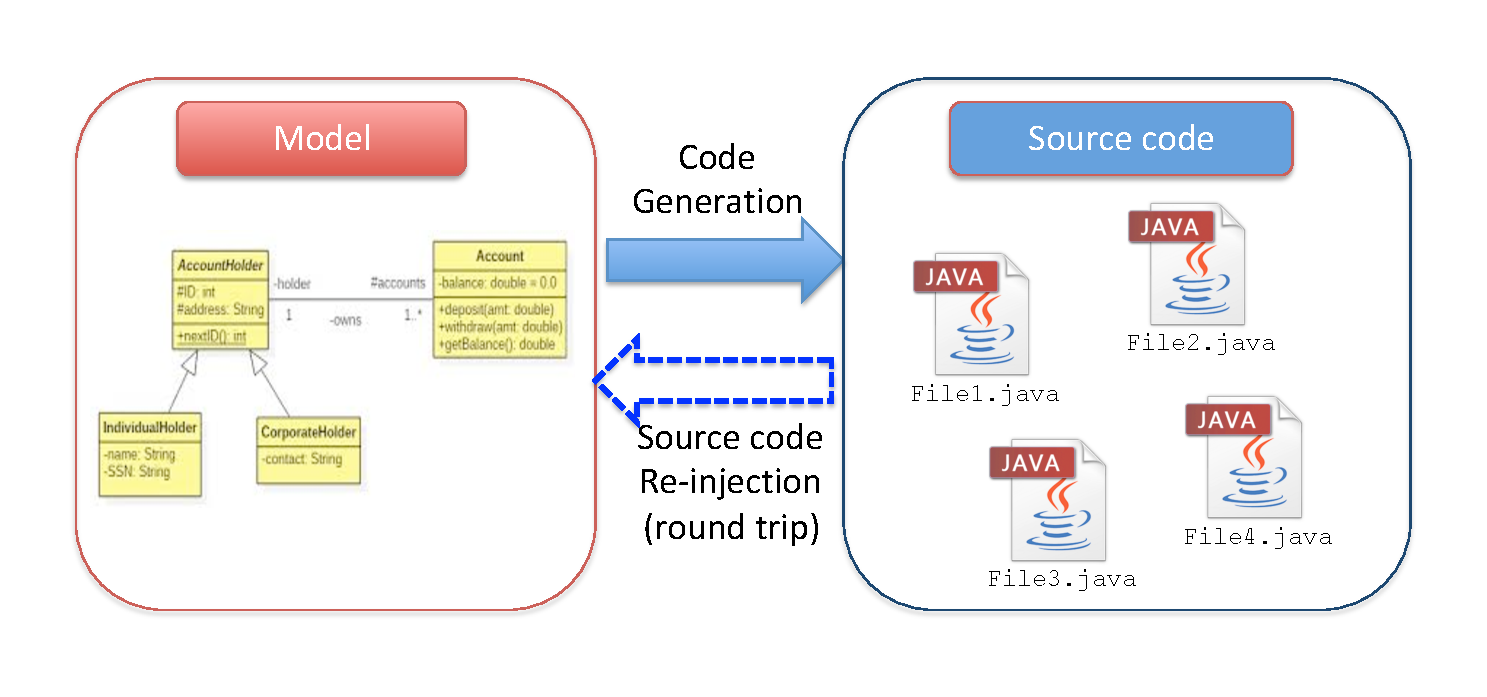
\includegraphics[width=1.0\columnwidth]{ClassicalVision.pdf}
    \caption{Classical vision for Model-Driven Engineering}
    \label{fig:ClassicalVision}
\end{figure}

Conversely, we propose a shift in the modeling paradigm in which models and code are developed together and at the same time in what we call a continuous modeling process. The PAMELA framework supports this paradigm shift by providing the means to: 
% Joel 1) annotate Java code with model-based annotations; 
%and 2) interpret these annotations at runtime.
1) weave model-based annotations with Java source code
and 2) interpret model annotations at run-time.

%\todo[inline]{In some sense we are loosing some of the advantages of modeling, aren't we? But let's see what reviewers say.}

% On peut éventuellement supprimer ce paragraphe
The rest of the paper is organized as follows. Section \ref{sec:pamproc} describes our approach and its associated development process. Section \ref{sec:architecture} presents the main building blocks of the PAMELA framework together with an illustrative example. Implementation details are discussed in Section \ref{sec:implementation}, followed by a description of industrial experimentation and validation cases in Section \ref{sec:validation}. We end the paper in Section \ref{sec:related} by discussing related work.


\section{Approach and Development Process}
\label{sec:pamproc}
We advocate for a strong coupling between model and sources code, to give architects and developers a way to both interact during the whole development cycle. PAMELA is an annotation-based Java modeling framework providing a smooth integration between model and code, without code generation nor externalized model serialization. Instead of generating the code, the API (mostly Java interfaces with abstract method declarations) is locally executed (interpreted). The idea is to avoid separation between modeling and code to facilitate consistency management and to /avoid round-trip issues. Figure \ref{fig:PamelaVision} summarizes the PAMELA architecture and is more detailed thereafter.  

\begin{figure}
    \centering
    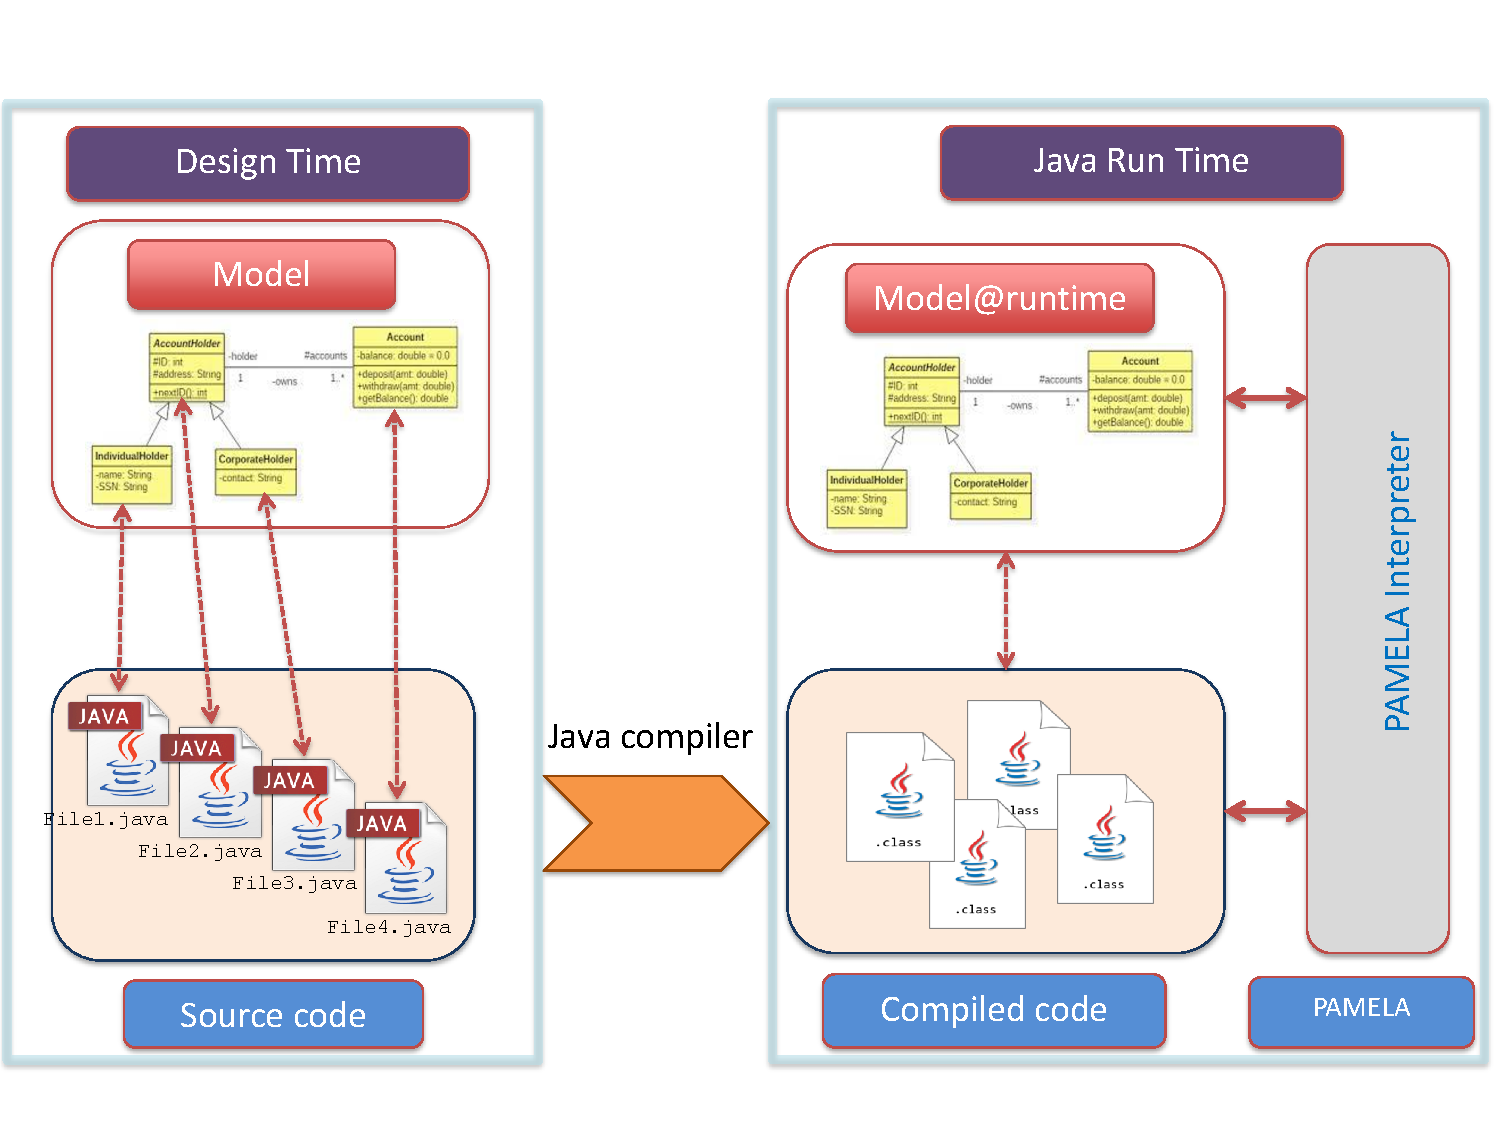
\includegraphics[width=1.0 \columnwidth]{PamelaVisionV2.pdf}
    \caption{PAMELA approach for modeling}
    \label{fig:PamelaVision}
\end{figure}

%\subsection{PAMELA Modeling/Development Process}

Coupling model and code into the same artifact opens new ways of programming. The classical (metadata enabled) programming process relies on \emph{programmers} that produce code reusing pre-existing modeling concepts. These concepts are implemented by \emph{modelers} that provide the right annotations the programmers use. This is, for instance, the process followed by Jakarta EE (JEE) developers reusing JEE specific annotations. The evolution rhythm between models and code is low. This programming way is still possible with PAMELA, but we allow the ability to reach a high evolution rhythm when the programmer also becomes the modeler. In fact, when the programmer identifies a pattern, an abstraction, a generalization, s/he can use PAMELA to develop and capitalize on this abstraction by increasing PAMELA metamodel. 

% Je pense qu'ici il faudrait plutot parler du modèle. Le métamodèle PAMELA est celui représenté figure 3. Ou alors parler du metametamodele PAMELA

The developed metamodels are implemented by annotations that rely on Java/JVM entities and mechanisms. They include consistency checking, which constrain their use and helps the programmer to avoid inconsistencies or errors. We have first experimented their use with setter/getter to define POJO entities, with traits to implement multiple inheritance or with roles and rules to set security rules on classes.

Our experience shows that introducing and reusing new concepts (1) reduce the size of the code (2) reduce the risk of errors and (3) improve the code structure. The cycle of development between the model and the code can then be drastically reduced, leading to what we call \emph{continuous modeling}.

The code size is reduced because abstractions factorize recognized concepts so that the code using such concepts is replaced by the use of the abstraction at the right place. This also reduces the risk of errors since the code is now managed by the PAMELA framework with all the required checks. Finally, the code structure is improved since it matches the way the programmer conceptualizes (models) her/his code.

Here are various conceivable scenarios for PAMELA use:
\begin{itemize}
    \vspace{-0.2cm}\item \textbf{Programming use} : programmers reuse existing annotations and write model and code at the same time (the modelers and programmers share the same artifacts : the Java code). This scenario includes the case where the model (made by the modelers) is pre-existing.
    \vspace{-0.2cm}\item \textbf{Reengineering} : programmers start from an existing code base (legacy) and refactor it while replacing this code by abstract method declarations in Java interface, reducing risks of errors.
    \vspace{-0.2cm}\item \textbf{Aspect-oriented programming} : programmers may use or redefine "patterns" (e.g., Security Patterns \cite{silva20}) which offers code weaving at runtime, and runtime monitoring.
    \vspace{-0.2cm}\item \textbf{Advanced programmers use} : programmers may extend PAMELA with their own annotations, implementations or patterns.
\end{itemize}

In this presentation, we focus on the programming use of PAMELA, when programmers reuse existing annotations. The full power of PAMELA arises when programmers become modelers defining their own abstractions/annotations.



\section{Software Framework and Features}
\label{sec:architecture}
Figure \ref{fig:PamelaVision} summarizes the PAMELA architecture.  Basically, it is composed of one design time component (the PAMELA metamodel, plus a number of predefined annotations) presented in the next section and one run-time component (the PAMELA interpreter), described in the section \ref{sub:RunTime}.

\begin{figure}
    \centering
    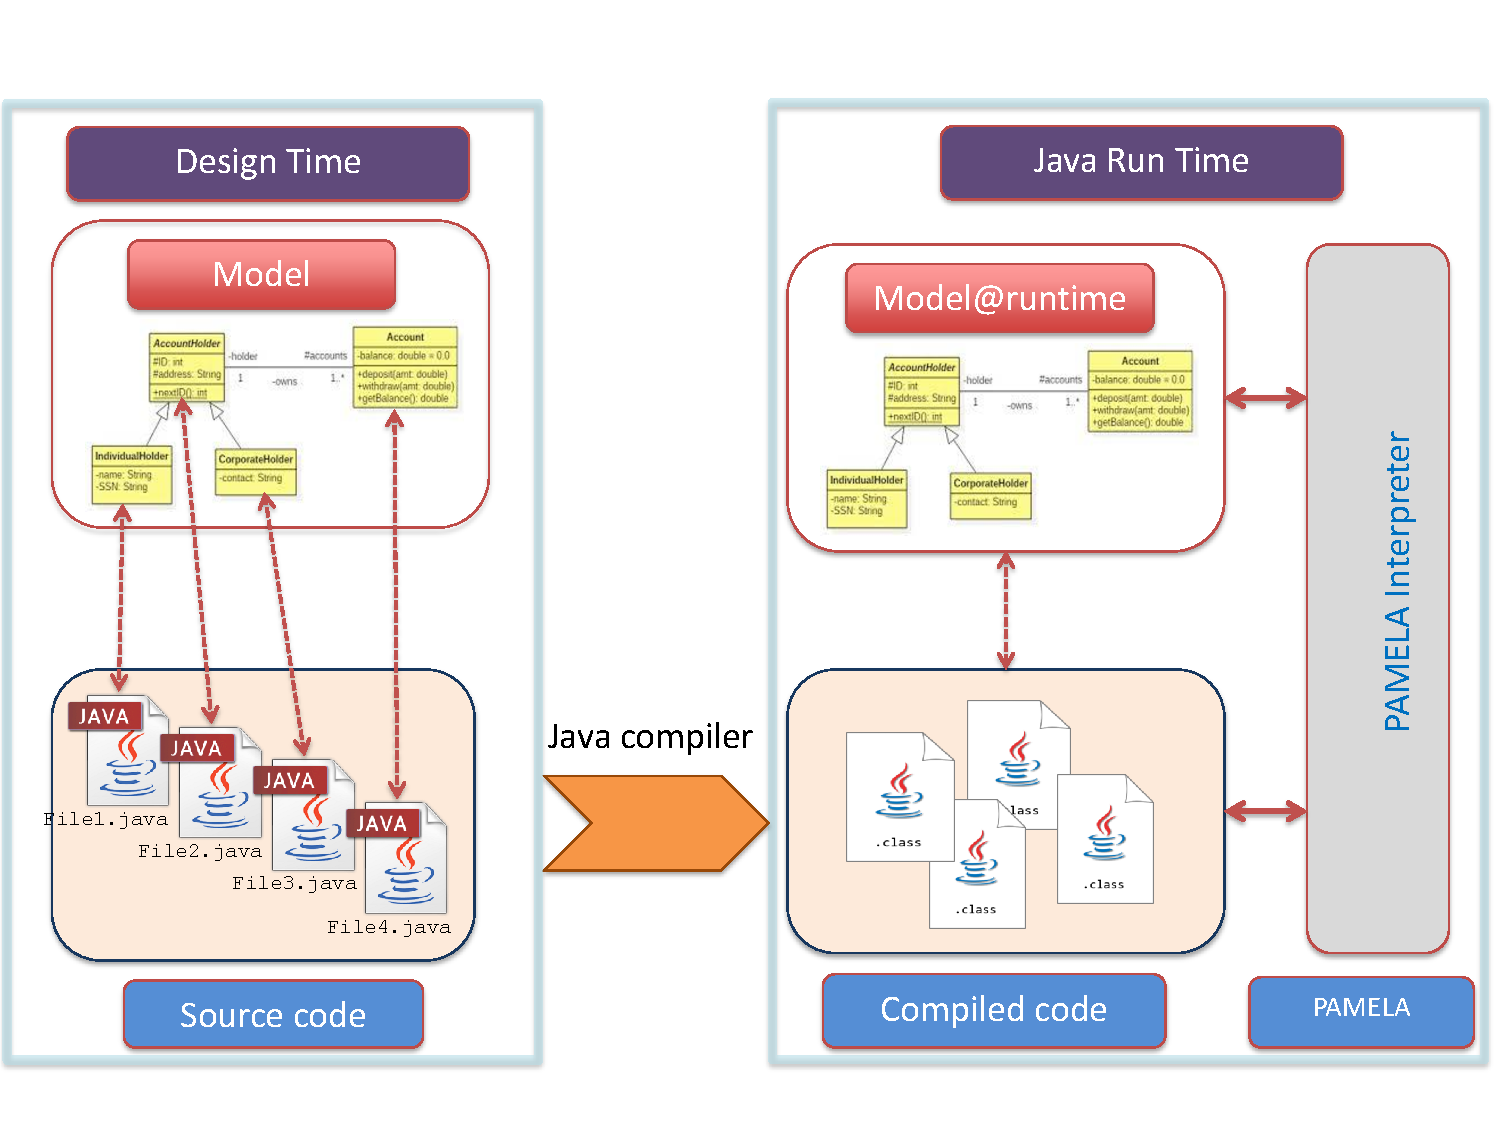
\includegraphics[width=1.0 \columnwidth]{PamelaVisionV2.pdf}
    \caption{PAMELA approach for modelling}
    \label{fig:PamelaVision}
\end{figure}


\begin{center}
\begin{figure}
    %\centering
    %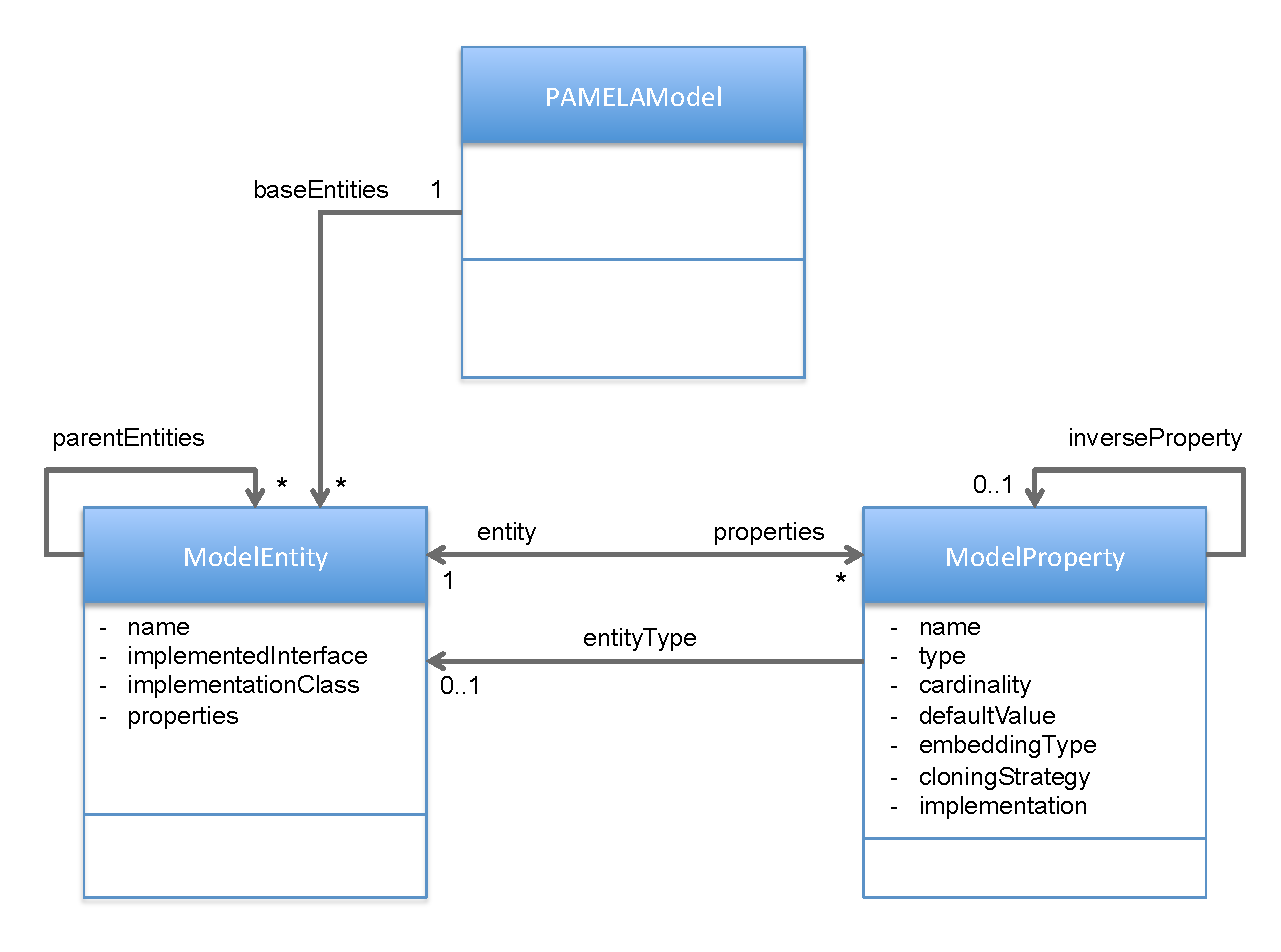
\includegraphics[width=1.0 \columnwidth]{PamelaMetaModel.pdf}
    \begin{tikzpicture}[scale=0.9]
    \useasboundingbox (-9,-5) rectangle (3,0);% ajustement à la main :-(
    \umlclass[x=-2,y=0]{PAMELAModel}{}{}
    \umlclass[x=-6,y=-3]{ModelEntity}{-- name \\ -- implementationInterface \\ -- implementationClass}{}
    \umlclass[x=2,y=-3]{ModelProperty}{-- name \\ -- type \\ -- cardinality \\ -- defaultValue \\ -- embeddingType \\ -- cloningStrategy \\ -- implementation }{}
    \umluniassoc[geometry=-|, arg1=baseEntities, mult1=1, pos1=0.45,  arg2=*, pos2=1.9]{PAMELAModel}{ModelEntity}
    \umluniassoc[arg1=entity, pos1=0.15, mult1=1, anchors=20 and 154, arg2=properties, mult2=*, pos2=0.75]{ModelEntity}{ModelProperty}
    \umluniassoc[anchors=154 and 20]{ModelProperty}{ModelEntity}
    \umluniassoc[mult1=entityType, pos1=0.5, arg2=0..1, pos2=0.9]{ModelProperty}{ModelEntity}
    \umluniassoc [arg=parentEntities , mult=*, pos=0.9, align= right, angle1=170, angle2=110, loopsize=2cm]{ModelEntity}{ModelEntity}
    \umluniassoc [arg=inverseProperty , mult=0..1, pos=0.9, align= left, angle1=20, angle2=80, loopsize=2cm]{ModelProperty}{ModelProperty}
    \end{tikzpicture}
    \caption{PAMELA metamodel}
    \label{fig:PamelaMetaModel}
\end{figure}
\end{center}
    
\subsection{Design time}
\label{sub:DesignTime}

The PAMELA metamodel is depicted in Figure  \ref{fig:PamelaMetaModel}, and allows, though the use of annotations, the definition of of \emph{simple} UML-like models directly on the code.

A \texttt{PAMELAModel} is defined as a set of references to \texttt{ModelEntity}. A \texttt{ModelEntity} reflects a concept and is encoded in a java \texttt{interface}. PAMELA metamodel allows multiple inheritance: thus \texttt{ModelEntity} may define a set of parent entities. Note that reification of \texttt{ModelEntity} is performed in a java \texttt{interface} (and not a class), which only defines API whithout any implementation for methods. 
Note that \emph{ModelEntities} may declare \emph{ImplementationClasses}, which will be responsible for providing custom code implementing domain or application specific behaviour. A partially implemented \texttt{abstract} java \texttt{class} may be defined as partial base implementation (conforms to implemented interface).

A \texttt{ModelEntity} also defines some properties, encoded as \texttt{ModelProperty}. A \texttt{ModelProperty} is identified by a name, a cardinality (simple or multiple) and a type, which can be a reference to another \texttt{ModelEntity}, or a Java type (a primitive or an arbitrary complex Java type). Depending on its cardinality, a \texttt{ModelProperty} is bound to a set of methods reflecting use of property.
\begin{itemize}
    \item A \emph{read-only single property} will define read-access of its value using a \emph{getter} (a java method defined in java interface taking no argument and returning desired value).
    \item A \emph{read-write single property} will define a \emph{getter} and a \emph{setter} (a java method taking value to be set as unique argument)
    \item A \emph{read-write multiple property} will define a \emph{getter}, an \emph{adder} (a java method taking value to be added as unique argument), a \emph{remover} (a java method taking value to be removed as unique argument), and may define additional methods for extended features such as reindexing for example.
\end{itemize}


To summarize, in the following we list the most common java annotations used in the context of \texttt{ModelEntity} and \texttt{ModelProperty} definitions:

\begin{itemize}
    \item \texttt{@ModelEntity}: tag annotating \texttt{interface} as \emph{ModelEntity}. May declare an abstract entity.
    \item \texttt{@ImplementationClass}: tag annotating \emph{ModelEntity} \texttt{interface} and precising abstract java \texttt{class} to be used as base implementation.
    \item \texttt{@Implementation}: tag annotating a partial implementation (abstract inner \texttt{class} defined in implemented \texttt{interface}), and used in the context of multiple inheritance.
    \item \texttt{@Getter(String)}: tag annotating method as unique getter for implicit \emph{ModelProperty} whose identifier is the declared String value. May also declares cardinality, enventual inverse property, default value and some other features.
    \item \texttt{@Setter(String)}: tag annotating method as unique setter for implicit \emph{ModelProperty} whose identifier is the declared String value.
    \item \texttt{@Adder(String)}: tag annotating method as unique adder for implicit multiple cardinality \emph{ModelProperty} whose identifier is the declared String value.
    \item \texttt{@Remover(String)}: tag annotating method as unique remover for implicit multiple cardinality \emph{ModelProperty} whose identifier is the declared String value.
    \item \texttt{@Reindexer(String)}: tag annotating method as unique reindexer for implicit multiple cardinality \emph{ModelProperty} whose identifier is the declared String value.
    \item \texttt{@Initializer}: tag annotating a method used as a constructor for related \emph{ModelEntity}
   \item \texttt{@Deleter}: tag annotating a method used as explicit destructor for related \emph{ModelEntity}
    \item \texttt{@Finder(String,String)}: tag annotating method as a fetching request for a given \emph{ModelProperty} with a given attribute
    \item \texttt{@CloningStrategy}: allows to customize cloning strategy for a given \emph{ModelProperty}
    \item \texttt{@Embedded}: allows to declare a given \emph{ModelProperty} as embedded according to PAMELA semantics
    \item \texttt{@Imports} and \texttt{@Imports}: allows to declare some entities to be included in PAMELA model
    \item \texttt{@XMLElement} and \texttt{@XMLAttribute}: used to specify XML serialization for PAMELA instances
    
\end{itemize}

 \subsection{Runtime}
 \label{sub:RunTime}
 
 The aforementioned models are executed at runtime as a combination of two components: 1) plain java byte-code, as the result of the basic compilation of source code; and 2) an embedded PAMELA interpreter, executing semantics reflected by \emph{ModelEntity} and \emph{ModelProperty}  declarations (together with custom annotations where available).

The main idea for the approach is to override java dynamic binding. Invoking a method on an object which is part of a PAMELA model, causes the real implementation to be called when existing (more precisely dispatch code execution between all provided implementations), or the required interpretation according to the underlying model to be executed. 
 
The PAMELA interpreter will intercept any method call for all instances of \emph{ModelEntity} and conditionally branches code execution.
 \begin{itemize}
     \item If the accessed method is part of a \emph{ModelProperty} (a getter, or a setter, etc..), and no custom implementation is defined neither in the class declared as implementation, nor in a class declared as partial implementation in the context of traits, then, execution is delegated to the related property implementation (generic code provided by the PAMELA interpreter).
     \item If the accessed method is defined in a class declared as implementation, or in a class declared as partial implementation, then this method is executed. The PAMELA API through the \mytexttt{AccessibleProxyObject} interface also provides access to generic behavior (super implementation), allowing the developer to define an overriding composition.
 \end{itemize}
 
This general scheme provides also an extension point allowing to instrument the code. This extension point is used in order to integrate other features such as notification management, undo/redo stack management, assertion checking at run-time (support for \emph{Design by Contract}, aka JML), and dynamic code weaving in the context of \emph{Aspect Programming}.

PAMELA model at runtime is computed dynamically, working on the classpath of launched java application, and starting from a simple java interface (or a collection of java interfaces) which is/are PAMELA-annotated. From a mathematical point of view, internal representation of the underlying model is a graph whose vertex are PAMELA \emph{ModelEntities} (annotated java interface), and edges are either inheritance links or reference links (a property whose type is another \emph{ModelEntity}. \mytexttt{@Imports} and \mytexttt{@Import} annotations allows to include some other \emph{ModelEntities} in the model. On the contrary, an annotation attribute \mytexttt{@Getter(...ignoreType=true)} allows to ignore the link. In that context, PAMELA model computation is a graph closure computation, starting from a collection of vertices\footnote{Model closure computation on-the-fly provides an interesting approach to deal with model fragmentation.}. A PAMELA model at runtime is represented by a \mytexttt{ModelContext}.

PAMELA instances (instances of \emph{ModelEntity}) are handled though the use of \mytexttt{ModelFactory}, which is instantiated from a \mytexttt{ModelContext}.

% Folloging section/itemize may be removed when needed 
%This composition offers many benefits: 
%\begin{itemize}
%    \item Strong coupling between model and code
%    \item Strong typing is kept, and required checks are performed by the java compiler
%    \item PAMELA framework provides interpretation of model@runtime
%    \item No need to generate POJO (plain old java objects), as their execution follow the standard semantics (less code, less bugs)
%    \item Custom implementation are provided if needed, using classical java extension points
%    \item It offers a way to intercept method calls and instrument the code
%    \item Assertions checking at runtime
%    \item Dynamic code weaving at runtime (aspect programming without compilation)
%\end{itemize}

\subsection{Additional Features}

PAMELA supports a number of advanced programming features (some already mentioned) such as:  multiple inheritance and traits, containment management, cloning, fine-grained notifications management, object graph comparison and diff/merge, visiting patterns, clipboard management, validation, support for \emph{design by contract} by integrating the Java Modeling Language (JML), Metaprogramming, Aspect Oriented Programming.


%A strong interest of the approach is that the model is encoded in java, and must be compiled. It forces the java compiler to perform required checks %for a PAMELA model encoded in a strong typed program. Execution semantics of model is fully compatible with Java semantics. Many validation rules %are automatically performed through classical java compilation, independently of underlying PAMELA execution semantics.

\subsection{Example}

Listing \ref{lst:model} shows a very basic model with two entities: \emph{Book} and \emph{Library}. Entity \emph{Book} defines two read-write single properties \emph{title} and \emph{ISBN} with single cardinality and with \texttt{String} type. Entity \emph{Book} also defines a constructor with initial \emph{title} value. Entity \emph{Library} defines a read-write multiple properties \emph{books} referencing \emph{Book} instances. Note that this code is sufficient to execute the model, while no additional line of code is required (only java interfaces and API methods are declared here). 

%\begin{figure}
%    \centering
\begin{lstlisting}[language=Java,basicstyle=\ttfamily\footnotesize, caption=Model creation, label=lst:model]
@ModelEntity
public interface Book extends AccessibleProxyObject {

  @Initializer
  public Book init(@Parameter("title")String aTitle);
  
  @Getter("title")
  public String getTitle();
  
  @Setter("title")
  public void setTitle(String aTitle);
  
  @Getter("ISBN")
  public String getISBN();
  
  @Setter("ISBN")
  public void setISBN(String value);
}

@ModelEntity
public interface Library extends AccessibleProxyObject {

  @Getter(value = "books", cardinality = Cardinality.LIST)
  public List<Book> getBooks();

  @Adder("books")
  public void addToBooks(Book aBook);

  @Remover("books")
  public void removeFromBooks(Book aBook);

  @Reindexer("books")
  public void moveBookToIndex(Book aBook, int index);
  
  @Finder(collection = "books", attribute = "title")
  public Book getBook(String title);
}
\end{lstlisting}
 %   \caption{A basic PAMELA model with two entities \texttt{Library} and \texttt{Book}}
 %   \label{fig:ABasicPamelaModel}
%\end{figure}

The execution and the management of this model may be performed using the following simple lines of code:

%\begin{figure}
%    \centering
\begin{lstlisting}[language=Java,basicstyle=\ttfamily\footnotesize, caption=model execution/manipulation, label=lst:execution]
// Instantiate the meta-model
// by computing the closure of concepts graph
ModelContext modelContext 
    = ModelContextLibrary.getModelContext(Library.class);
// Instantiate the factory
ModelFactory factory  = new ModelFactory(modelContext);
// Instantiate a Library
Library myLibrary = factory.newInstance(Library.class);
myLibrary.setName("My library");
// Instantiate some Books
Book myFirstBook 
    = factory.newInstance(Book.class, "Lord of the ring");
Book anOtherBook = factory.newInstance(Book.class, "Holy bible");
myLibrary.addToBooks(myFirstBook);
myLibrary.addToBooks(anOtherBook);
\end{lstlisting}
 %   \caption{Executing a PAMELA model}
 %   \label{fig:ExecutingPamelaModel}
%\end{figure}

The first line of code instantiates a \texttt{ModelContext} by introspecting and computing the closure of concepts graph obtained while starting from \texttt{Library} entity and following \texttt{parentEntities} and \texttt{properties} relationships. This call builds at runtime a \emph{PAMELAModel}, while dynamically following links reflected by compiled byte-code. A factory \texttt{ModelFactory} is then instantiated using that \texttt{ModelContext}, allowing to create \emph{Library} and \emph{Book} instances.

Custom code can be easily added to this model as we show in Listing \ref{lst:custom}. It shows how to integrate custom code to the fully interpreted \emph{Book} entity described above. The partial custom implementation is offered by a partial class (note the \texttt{abstract} keyword), declared in the annotation header of model entity. Custom implementations are defined using classical java implementation/overrides scheme. Here we define the implementation of the \texttt{read()} method, which has no annotation (and thus, can not be processed by the PAMELA framework), and also the implementation of a custom getter for \emph{title}, returning a default value when no value is defined for that property. Note that this implementation references a default interpretated implementation (call to \texttt{performSuperGetter(String)} method).

%\begin{figure}
%    \centering
\begin{lstlisting}[language=Java,basicstyle=\ttfamily\footnotesize,caption=Custom Code, label=lst:custom]
@ModelEntity
@ImplementationClass(BookImpl.class)
public interface Book extends AccessibleProxyObject {

  static final String TITLE = "title";

  @Getter(TITLE)
  String getTitle();
  // ... title property declarations ...

  void read();
}

// Provides a partial implementation for Book
public static abstract class BookImpl implements Book {

  @Override
  public String getTitle() {
    String title = performSuperGetter(TITLE);
    if (title == null) {
      return "This book has no title";
    }
    return title;
  }

  @Override
    public void read() {
      // do the job
    }
}
\end{lstlisting}
 %   \caption{Executing a PAMELA model}
 %   \label{fig:ExecutingPamelaModel}
%\end{figure}


\section{Implementation}
\label{sec:implementation}
The PAMELA implementation is available online\footnote {\url{https://github.com/openflexo-team/pamela}}.

\subsection{Exposed API at design-time}

The model-code integration we advocate requires facilities to encode metadata in the source code. This requires an annotation-enabled language. Such a language supports the attribute-oriented programming if its grammar allows adding custom declarative tags to annotate standard program elements. Java programming language is a good candidate, as it supports annotations.

The PAMELA API exposed to the developer mainly consists of : 1) a set of annotations; and 2) a set of unimplemented Java interfaces exposing required features.

The package \texttt{org.openflexo.pamela.annotations} package exposes the set of annotations which were presented in Subsection \ref{sub:DesignTime}.

The package \texttt{org.openflexo.pamela} contains the following feature-related Java interfaces:
\begin{itemize}
    \item \texttt{AccessibleProxyObject} is the interface that PAMELA objects should extend in order to benefit from base features such as generic default implementation, containment management, notification, object graph comparison and diff/merge, visiting patterns, etc.
    \item \texttt{CloneableProxyObject} exposes features related to cloning.
    \item \texttt{DeletableProxyObject} exposes features related to deletion management.
    \item \texttt{SpecifiableProxyObject} exposes dynamic assertion checking features in the context of JML (contract management) use. 
\end{itemize}

% Generic design patterns API, used in the context of aspect programming is exposed in \texttt{org.openflexo.pamela.patterns} package. A plug-in architecture allows to enrich model with some specific design pattern. Some basic design patterns are released with PAMELA 1.6.x in the context of security (Authenticator, Authorization, SingleAccessPoint, Owner).

\subsection{PAMELA interpreter}

The package \texttt{org.openflexo.pamela.factory} contains the PAMELA interpreter implementation. The core of the interpreter is implemented in the class \texttt{ProxyMethodHandler}.

From a technical point of view, PAMELA implementation uses the \emph{javassist} reflection library (see \cite{shigueru2000}) which provides the \texttt{MethodHandler} mechanism, which is a way to override the Java dynamic binding. Invoking a method on an object which is part of a PAMELA model, causes the real implementation to be called when existing (more precisely dispatch code execution between all provided implementations), or the required interpretation according to underlying model to be executed. This provides also an extension point allowing to instrument the code, which is used for other features such as undo/redo stack management, and assertion checking at run-time (support for Design by Contract, aka JML).

The PAMELA framework is a 100\% pure Java ($\geq$ /1.81.8), compilable by a classical Java compiler and executable in a classical Java Virtual Machine.

\subsection{PAMELA code base metrics}

\sg{

PAMELA implementation is modularized. 

\begin{itemize}
    \vspace{-0.2cm}\item Core implementation (\texttt{pamela-core}) provides all base features for PAMELA. It contains 20k lines of code involving 184 classes. This code is covered with unit test (6k lines of code, 112 classes). Reached code coverage is about 66\%.
    \vspace{-0.2cm}\item \texttt{pamela-security-patterns} is an add-on library containing some security-pattern implementations.
    \vspace{-0.2cm}\item \texttt{pamela-perf-tests} contains benchmarking tools whose purpose is to quantifiate PAMELA performances. 
\end{itemize}

}
%\todo{Surely you can say more about its structure, size of components, ... other interesting and relevant observations on the codebase?}

\subsection{On performance issues}

\sg{
Compared to a basic POJO (Plain Object Java Object) implementation, use of PAMELA involves a significant CPU and memory-footprint overhead, because of the partially-interpretated nature for some model features.

A workbench\footnote {\url{https://github.com/openflexo-team/pamela/tree/1.6.1/pamela-perf-tests}} has been developped to help measure that overhead. We use a base model composed of four entities defining 4 to 5 properties (single and multiple properties), and we instantiate that tree model (1010101 objects created and initialized to default value). From this simple model, two java implementations have been derived using code generation. The first implementation was made using fully implemented java classes (POJO), while the second one is fully interpretated (it uses PAMELA framework and defines only interfaces and API methods). 

Unsurprisingly, we quantifiate a significant CPU overhead (from x20). This is due to the fact that \texttt{MethodHandler} mechanism is fully interpretated and contains many hooks, and cannot be compared to a fully-compiled and optimized Java dynamic binding. As well, memory footprint is increased from a x5 factor.

These conclusions must be moderated by the fact that this overhead only applies to a very small portion of code (mostly property accessors methods). A "real-world" model implementation generally involves a bigger "business code" part, which is generally the first CPU-time consumer. Using PAMELA won't increase CPU use on "business code" if this code is implemented with plain Java code (which is generally the case). As we will see in next section, PAMELA has been successfully applied to many industrial projects, where no major performance issues were reported.

Moreover, comparison between the two implementations should be tempered by the fact that PAMELA implementation offers many functional features which are not present in the base implementation (such as undo/redo, clipboard management, runtime monitoring and weaving, etc...).

}

% Rajouter un paragraphe sur le fait que PAMELA est une implementation du MOP (meta object protocol) ?

% Is it the good place for following links ?
%https://pamela.openflexo.org
%https://github.com/openflexo-team/pamela





\section{PAMELA industrial use cases and experiments}
\label{sec:validation}

 The PAMELA framework has been successfully applied in a variety of complex programming and modeling scenarios and we continue to use it daily as part of our modeling toolbox. In the following, we describe three important use cases in which PAMELA was a core component.

%\todo[inline]{General comment: I would change the title of the section to something like, Pamela Use cases, Pamela success stories or something of the like. The idea here is to show that pamela is a tool that is used and solve problems. In that sense, the fact that pamela powers Open flexo should be highlighted. In the same sense, the importance of the patterns and security should be reduced and limited to the fact that pamela allows it (the point being, to cite the workshop paper). I believe giving details of how patterns are implemented  here will distract the reader. technical details, if needed would be better placed in the implementation section.}

%https://pamela.openflexo.org
%https://github.com/openflexo-team/pamela

\subsection{Openflexo infrastructure}

Model Federation~\cite{Golra2016} is an approach that provides the means to
integrate multiple models conforming to different paradigms, and giving to each
stakeholder a specific view adapted to its needs. Model federation approach is
developed as a possible response to SIMF RFP (Semantic Information Modeling for
Federation)~\cite{simf-rfp} by OMG (Object Modeling Group). This RFP (Request For Proposal)
requests submissions for a standard addressing ”federation of information
across different representations, levels of abstraction, communities,
organizations, viewpoints, and authorities”. Thus model federation allows the
integration of heterogeneous models to develop new cross-concern
viewpoints/models or to synchronize the models used for designing a system. 

Openflexo\cite{OpenflexoWebSite} is a software infrastructure providing support
for model federation across multiple technological spaces. Conceptualization is
addressed through the proposition of a language called FML (Flexo Modeling
Language), which is executable on the platform. Openflexo infrastructure
introduces connectors (also called Technology Adapters) to support various
technological spaces and paradigms.

This open source initiative is now mature at the infrastructure level, and many
projects and applications have been developed and powered using Openflexo
infrastructure. More than 15 technology adapters have been developed, with
various maturity stage regarding their industrialization (Microsoft Word, Excel
and PowerPoint, EMF, OWL, Diagraming, JDBC, XML, OSLC, etc.)

The full Openflexo infrastructure is composed of about 50 components. In most components, the PAMELA framework is largely used. As an example the \texttt{diana} component\footnote{\url{https://diana.openflexo.org}} (a component providing diagraming features) is composed of 998 classes. 159 of those classes (mostly the diagraming model) are defined as Pamela \texttt{ModelEntity}. 

The total base of code for Openflexo infrastructure represents around
\num{900000} lines of Java code. Regarding backend modeling, the PAMELA
framework is extensively used in Openflexo core as well as in most technology
adapters, with very few specific implementations for properties. The
observer/observable pattern is generally used for graphical user interfaces,
which also rely on the PAMELA framework. 

An interesting experiment has been done in the context of Openflexo development process. When PAMELA was integrated to the code base, a big portion of the former legacy code has gradually and iteratively been migrated to PAMELA. Refactoring mainly consisted in removing code, and replacing method implementation by API method declaration. In some parts of core model implementation, code has been reduced by 80\% (in terms of lines of Java code), and many bugs disappeared, as they were caused by programming errors.

The PAMELA implementation is now really stable and mature. According to Openflexo infrastructure developers, maintenance of code base (about 10 years of development) raises no PAMELA-specific issue, while co-evolution of models and code is greatly improved compared to a 'code generation'-based solution.

% Continuous integration ?

\subsection{Formose project}

The Formose ANR (French National Agency for Research) project
(ANR-14-CE28-0009)\cite{FormoseWebSite} aimed to design a formally-grounded,
model-based requirements engineering (RE) method for critical complex systems,
supported by an open-source environment. The main partners were: ClearSy, LACL,
Institut Mines-Telecom, OpenFlexo, and THALES. 

The main results of the project are a requirements modeling multi-view
language, its associated design process and the development of an open-source
platform called Formod\cite{FormodWebSite}, built using Openflexo
infrastructure and the PAMELA framework. %\todo{Say how and where PAMELA was used}
The requirements modeling language is based on KAOS~\cite{kaos} for goal
modeling and SysML for the structural part of a system. The associated domain
modeling language, used to describe system domain knowledge, extends the two
ontology languages OWL~\cite{owl} and PLIB~\cite{plib}. The graphical notations
are then translated into Event-B~\cite{eventb}, a formal specification method supported by verification tools. 

%\todo{Remark that it is industry ready}

The Formose method and Formod tool have been evaluated on different case studies provided by the industrial partners of the project.



\subsection{SecurityPatterns experiment}

A significant experiment in PAMELA is the implementation of security patterns weaved on domain code \cite{silva20}.
In this context, the PAMELA framework is extended to include the notion of Pattern, i.e. a composition of multiple classes. Included to this experiment, the security pattern is specified by expected behavior defined and formalized by a pattern contract. This contract is defined by formal properties and the PAMELA framework ensures the property verification at runtime.

Related to the security pattern implementation, PAMELA enables the definition of additional security behavior to existing Java code.
Patterns are defined in PAMELA using three classes, each one representing a different conceptual level \texttt{PatternFactory}, \texttt{PatternDefinition}, \texttt{PatternInstance}.

To declare a Pattern on existing code, pattern elements such as Pattern Stakeholders and methods need to be annotated with provided security pattern-specific annotations. These annotations will be discovered at runtime by the \texttt{PatternFactory} and stored in \texttt{PatternDefinition} attributes.


Summarizing, implementing Patterns with PAMELA provides the ability to monitor the execution of the application code; the ability to offer extra structural and behavioral features, executed by the PAMELA interpreter; a representation of Patterns as stateful objects. Such objects can then evolve throughout runtime and compute assertions.





%\subsection{Performance issues}

% parler des problèmes de perfs

%\subsection{Syntaxic issues}

% Problème d'un truc trop verbeux > editeur graphique

\label{sec:Experimentations}


\section{Related Work}
\label{sec:related}
Very few approaches build interfaces between MDE artifacts and source code at runtime. FAME \cite{kuhn2008fame} is  a library that keeps metamodels accessible and adaptable at runtime. Basically, FAME attaches meta-information to the objects of a running application permitting an uniform manipulation of both models and system objects at runtime. Similarly, in \cite{song2010applying} the authors use runtime models to maintain a causal connection between a model and a running systems for monitoring and control purposes. More recently, in \cite{boronat2019} the authors construct and maintain at runtime model-based views on the data manipulated in object-oriented code. Different to the aforementioned approaches, PAMELA does not focus in reflecting and manipulating running systems but in: 1) extending their behaviors; and 2) maintaining a continuous cycle of metamodeling so that models and corresponding code remain synchronized without the need for code generation processes. In a different approach, UMPLE \cite{lethbridge2016merging} mixes programming and modeling by integrating UML constructs into languages such as Java. However, they use code generation for the runtime part of the system.


\section{Conclusion}

The PAMELA framework promotes a modeling paradigm where models and code are jointly developed to provide a continuum between model and source code. The support is supplied by Java annotations and the PAMELA interpreter at runtime.

The different experiments provide efficient examples to argue the benefits of
the PAMELA framework but it is better to make your own experiences through \url{https://pamela.openflexo.org/}.



%%
%% The next two lines define the bibliography style to be used, and
%% the bibliography file.
\bibliographystyle{ACM-Reference-Format}
\bibliography{biblio}

\end{document}
\endinput
%%
%% End of file `sample-sigchi.tex'.

% Test
